% !TeX spellcheck = en_GB 
\documentclass{article}

\usepackage{amsmath} % Advanced math typesetting
\usepackage[utf8]{inputenc} % Unicode support (Umlauts etc.)
\usepackage[ngerman]{babel} % Change hyphenation rules
\usepackage{hyperref} % Add a link to your document
\usepackage{graphicx} % Add pictures to your document
\usepackage{listings} % Source code formatting and highlighting
\usepackage{babelbib}
\lstset{
	columns=fullflexible,
	frame=single,
	breaklines=true
}
\newcommand{\quotes}[1]{``#1''}
\begin{document}
\section*{CMPT 406 Final Project Report}
\paragraph{Name:} Ruijia Mao
\paragraph{SFU ID:} 301295769
\subsection*{1. Problem Definition}
Given a set of random points on the surface of a sphere, we want to calculate the spherical Voronoi diagram on the sphere. Then, we want to get a \quotes{good} spherical Voronoi diagram based on that. Without loss of generality, we will calculate the Voronoi diagram on a \textbf{unit sphere}, which is defined by
\begin{equation}
\{\ p\ |\ p \in \mathbf{R}^3, ||p||_2 = 1\ \}
\end{equation}
Also, the \textbf{distance function} we used to calculate the distance between two points on the surface of a sphere is geodesic distance, which is defined by the arclength of the shorter segment of the great circle that passes through two points. We will use $d(p, q)$ to denote the geodesic distance between two points $p$ and $q$ on the surface of a sphere. 
\subsection*{2. Literature Review}
Currently, there are two methods for constructing the spherical Voronoi diagram. One is through convex hull[1]. The other is through plane sweep[2]. The algorithm we used in this project is the first method. Because I've talked about those methods in the presentation session, I won't elaborate the details of them here. 
\\
\subsection*{3. Method}
We want to generate a \quotes{good} spherical Voronoi diagram in this project. The method I used is referenced from a website[3] talking about polygon map generation. More specifically, For a specific region in a Voronoi diagram, I sum all the points in the region and normalize the sum. Because we are constructing the Voronoi region on a unit sphere, the point will be a point on the sphere. I will repeat the process until the points converge or the number of iteration reaches the limit which I set the limit to 300. The converge is defined by the state of the points appeared in previous iterations. 
\subsection*{4. Result}
The results are shown bellow. 
For small number of points on the sphere, say like 6 points,  the Voronoi points will converge in around 30 iterations. 
\\
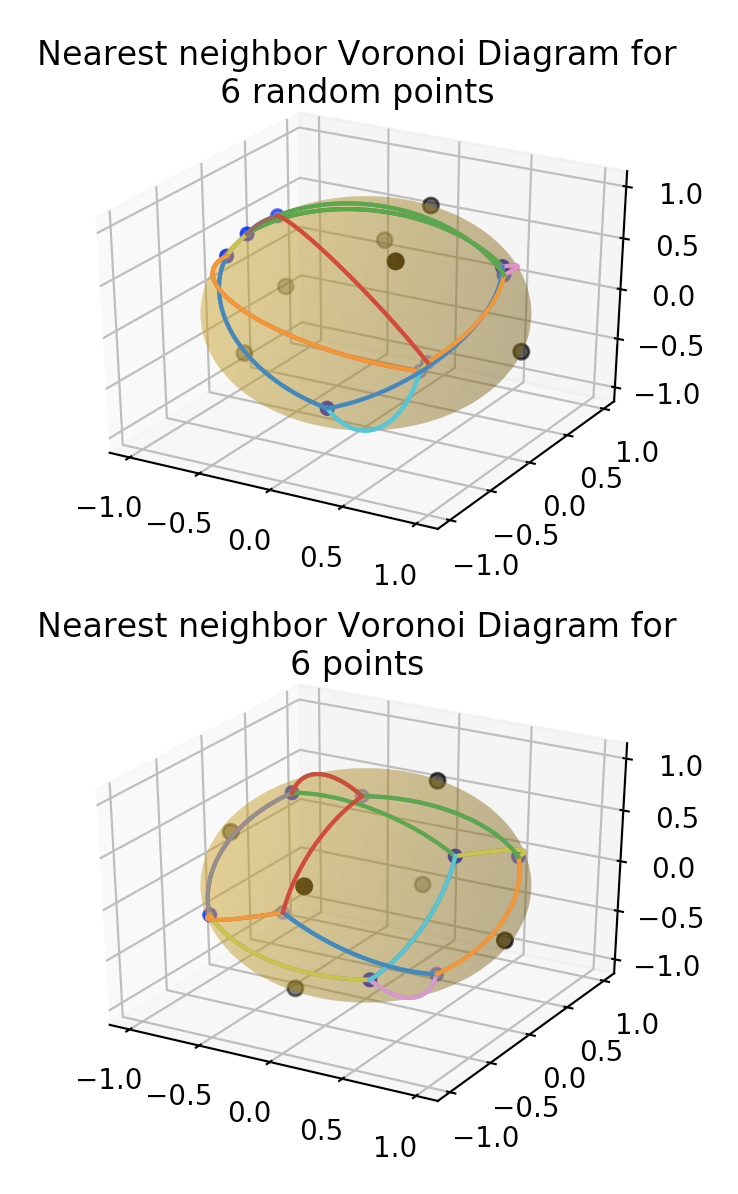
\includegraphics[scale=0.4]{v6}
\\
Basically, if we connect voronoi points with straight lines instead of curves, a cuboid will be formed. 
\\
For 10 points, it can converge with around 60 iterations. 
\\
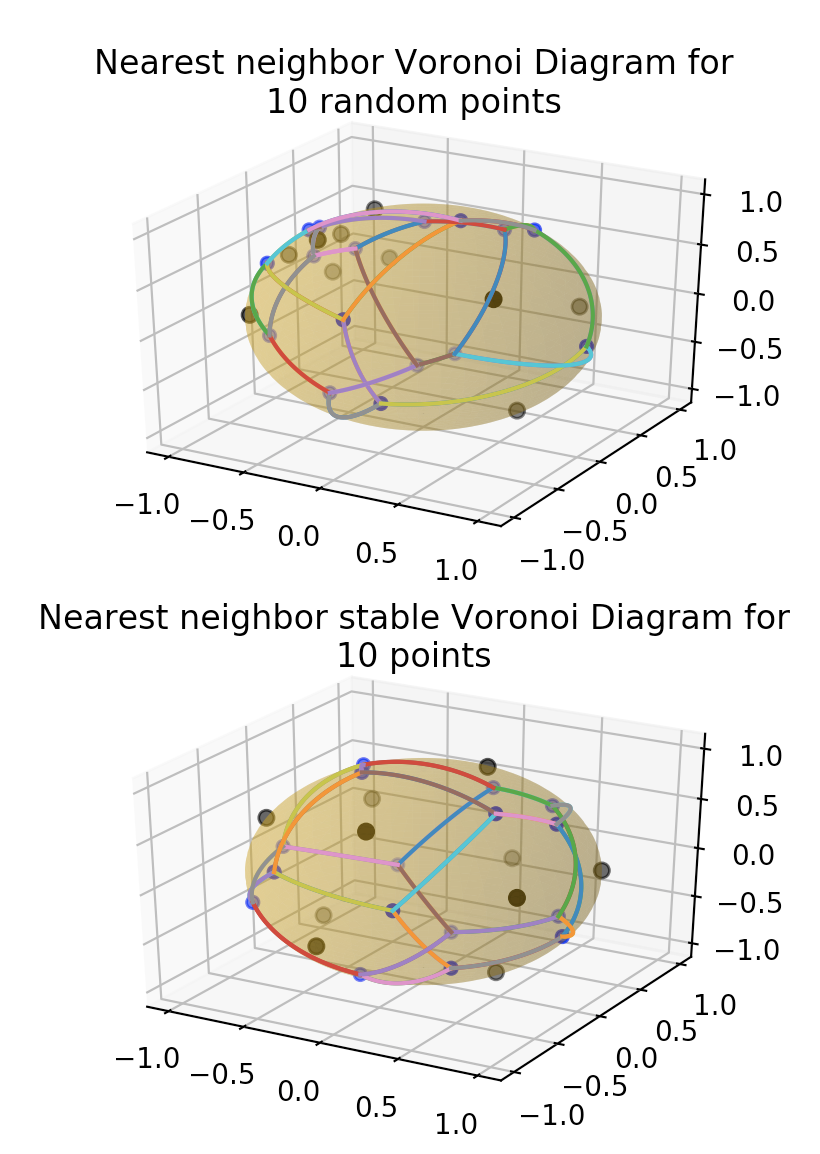
\includegraphics[scale=0.4]{v10}
\\
But with the random points, the points are less likely to converge. But the differences between iterations are minor.  For example, the following graphs shows the voronoi diagram of 50 points after 50 and 300 iterations. 
\\
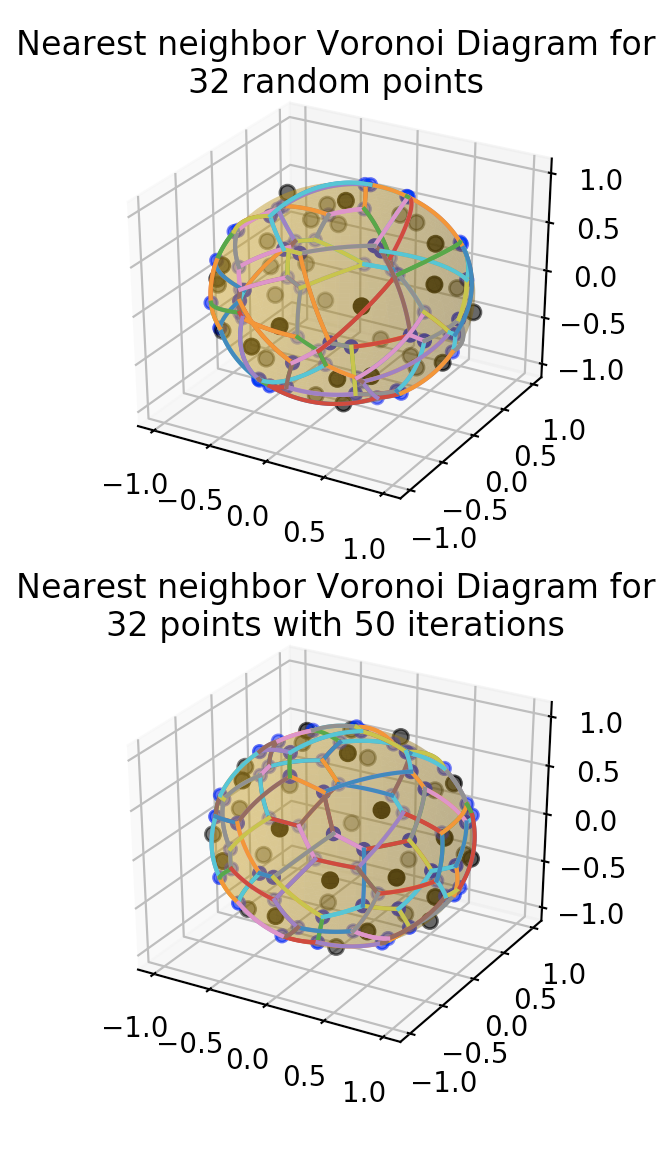
\includegraphics[scale=0.4]{v32_50}
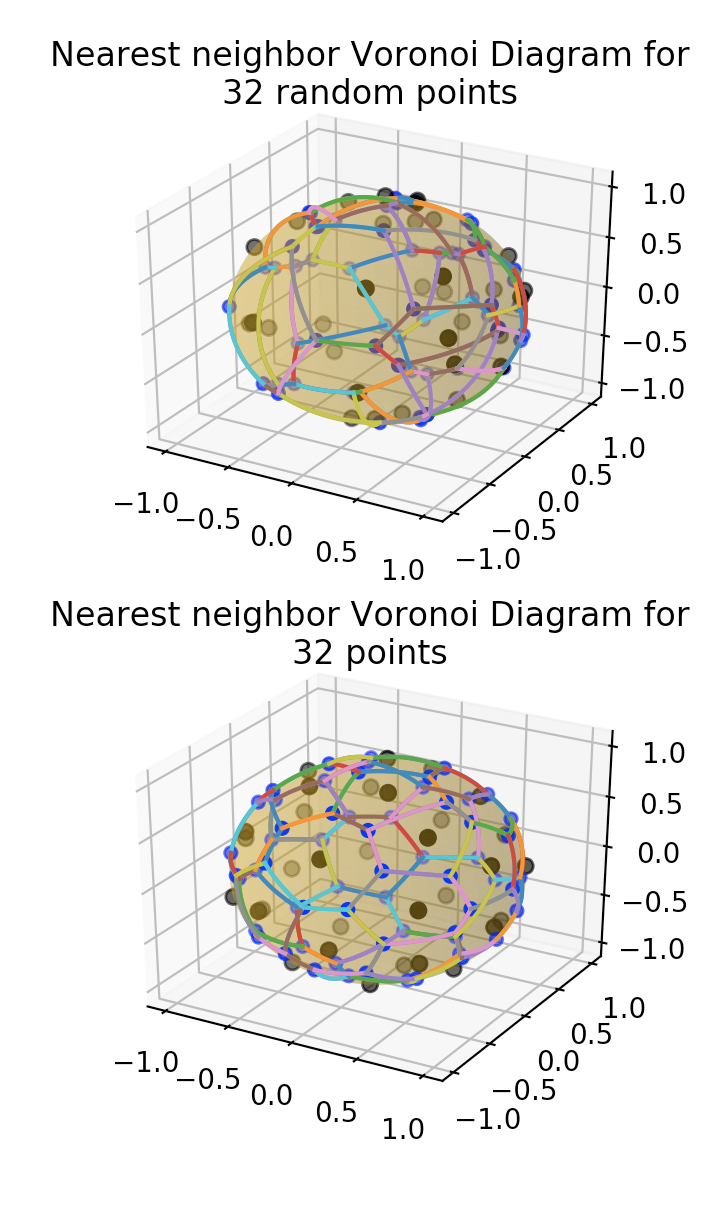
\includegraphics[scale=0.4]{v32}
\\
Also, furthest point Voronoi diagram can be constructed by using the diametrically opposite points and constructing the nearest neighbor Voronoi diagram for them. Here are some examples.
\\
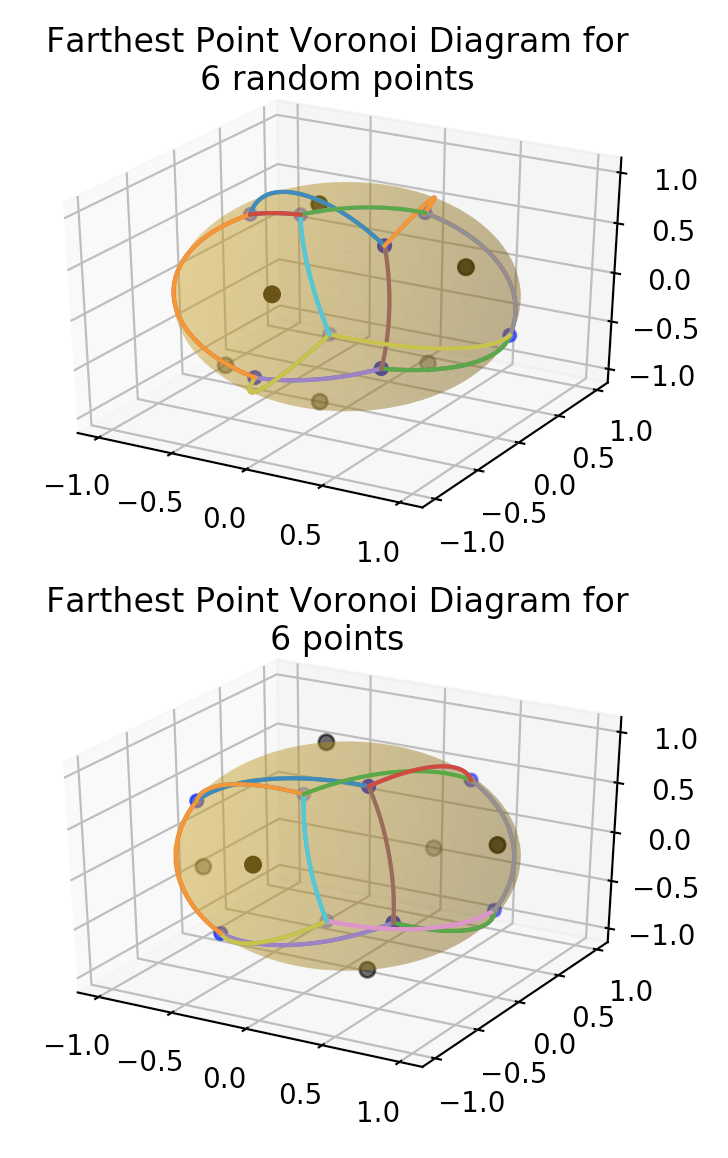
\includegraphics[scale=0.4]{f6}
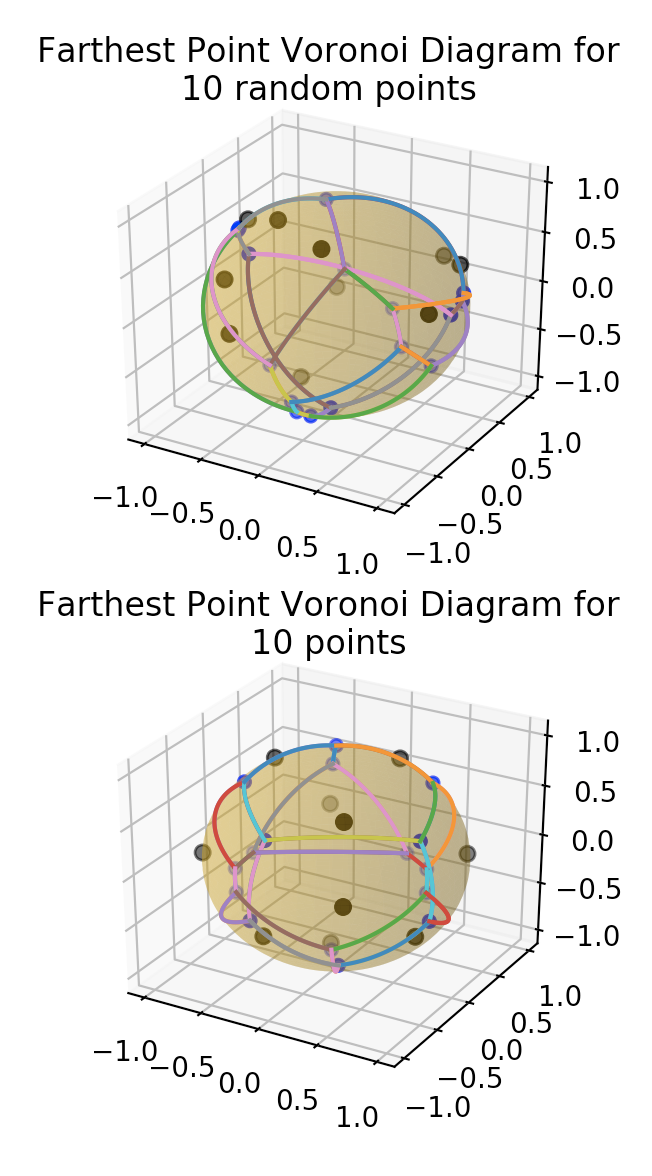
\includegraphics[scale=0.4]{f10}
\\
\subsection*{5. Future Work}
I think in the future, I can investigate the reason why when more points are considered, the Voronoi diagram does not converge. Current inspection suggests that the Voronoi points are moving along some specific directions. Another possible reason may be there are some subtle bugs in my program. 
\subsection*{6. Reference}
$[1]$ K. Q. Brown.Geometric transforms for fast geometric algorithms. Ph.D. thesis, Dept. Comput. Sci., Carnegie-Mellon Univ., Pittsburgh, PA, 1980. Report CMU-CS-80-101
\\ 
$[2]$ Zheng, X., Ennis, R., Richards, G.P., Palffy-Muhoray, P.: A plane sweep algorithm for the Voronoi tessellation of the sphere. Electron.-Liq. Cryst. Commun. 1 (2001).
\\
$[3]$ Amit Patel (2010, Sep 4). Polygonal Map Generation for Games. Retrieved from http://www-cs-students.stanford.edu/~amitp/game-programming/polygon-map-generation/
\end{document}